%File: main.tex
% AAAI 2027 submission draft, prepared with the AAAI 2026 author kit
% (per instruction: AAAI 2027 follows the AAAI 2026 format).
% ANONYMOUS SUBMISSION MODE IS ON:
\def\aaaianonymous{true}
%
\documentclass[letterpaper]{article} % DO NOT CHANGE THIS
\ifdefined\aaaianonymous
    \usepackage[submission]{aaai2026}  % Anonymous submission version
\else
    \usepackage{aaai2026}              % Camera-ready version
\fi
\usepackage{times}  % DO NOT CHANGE THIS
\usepackage{helvet}  % DO NOT CHANGE THIS
\usepackage{courier}  % DO NOT CHANGE THIS
\usepackage[hyphens]{url}  % DO NOT CHANGE THIS
\usepackage{graphicx} % DO NOT CHANGE THIS
\urlstyle{rm} % DO NOT CHANGE THIS
\def\UrlFont{\rm}  % DO NOT CHANGE THIS
\usepackage{natbib}  % DO NOT CHANGE THIS AND DO NOT ADD ANY OPTIONS TO IT
\usepackage{caption} % DO NOT CHANGE THIS AND DO NOT ADD ANY OPTIONS TO IT
\frenchspacing  % DO NOT CHANGE THIS
\setlength{\pdfpagewidth}{8.5in} % DO NOT CHANGE THIS
\setlength{\pdfpageheight}{11in} % DO NOT CHANGE THIS
\usepackage{booktabs}
\usepackage{amsmath}
\pdfinfo{
/TemplateVersion (2026.1)
}
\setcounter{secnumdepth}{0}

% Macros
\newcommand{\stage}[1]{\textsc{#1}}

\ifdefined\aaaianonymous
    \title{The Harness, Not the Hierarchy:\\What Governs Learned Guidance in Search-Based Planning}
    \author{Anonymous Submission}
    \affiliations{}
\else
    \title{The Harness, Not the Hierarchy:\\What Governs Learned Guidance in Search-Based Planning}
    \author{Anonymous Submission}
    \affiliations{}
\fi

\begin{document}

\maketitle

\begin{abstract}
We report a preregistered, thirteen-stage experimental program asking what governs the payoff of learned guidance in search-based planning: the \emph{harness}---representation, planner integration, information access, and supervision regime---or the architectural hierarchy of the model that produces the guidance. Hierarchical recurrent architectures are increasingly credited with planning ability, yet apparent wins and losses are routinely confounded by harness choices that are rarely controlled. On calibrated probabilistic-roadmap benchmarks (hard static suites, space--time dynamics, compositional missions, and bounded-observation planning) and a discrete-grid counterpart, we pair every architecture comparison with oracle headroom gates, matched-solved paired statistics, twin controls, and preregistered falsifiers. Learned guidance itself is large and real---15--48\% fewer A\textsuperscript{*} expansions on static suites and 62--95\% on dynamic suites---but every factor that governed it was a harness factor: a representation change rescues a collapsed model; the same frozen weights turn from inert to a 6--15\% win when moved from additive magnitude to focal ranking; low-rank adaptation plateaus by capacity, not by its output bound; and no hierarchy or depth-of-compute dose--response survives controlled testing, with learned halting \emph{anti-}correlating with mission depth ($\rho{=}-0.407$). Restructuring the harness rather than the architecture---bounded local observations plus one inference-time Bellman backup on a small flat MLP---beats every complete-map provider from the program's static benchmark on 144 held-out worlds, cutting expansions 15.95\% against the preregistered hierarchical comparator at matched empirical path quality.
\end{abstract}

\section{Introduction}

Learned heuristics promise to make search-based planners cheaper: replace a loose admissible estimate with a model that has seen thousands of solved problems, and A\textsuperscript{*} expands fewer nodes \citep{arfaee2011bootstrap,bhardwaj2017sail,yonetani2021neuralastar}. A prominent recent thread attributes such gains specifically to \emph{architectural hierarchy}: recurrent models with fast and slow modules and adaptive computation, exemplified by the Hierarchical Reasoning Model \citep[HRM;][]{wang2025hrm}, are argued to perform latent multi-step planning. Independent analyses have already begun to question how much of that performance the hierarchy itself explains \citep{jolicoeur2025trm}.

This paper reports what happened when we set out to \emph{confirm} the hierarchy account on planning benchmarks and instead falsified it---informatively. Across a thirteen-stage continuous program (\stage{C1}--\stage{C13}) on probabilistic-roadmap (PRM) planning \citep{kavraki1996prm} and a parallel discrete grid program, every factor that determined whether learned guidance paid off sat in what we call the \emph{harness}: (i) the \emph{representation and training objective} given to the model, (ii) the \emph{integration point} at which its output enters the planner, and (iii) the \emph{information access, task formulation, and supervision regime} it is trained under. None sat in nominal hierarchy. Where architectures did separate, the winners were models with the right \emph{global or local information structure} (a U-Net over the map, a graph network over the product graph), at specific regimes, and never with a growing advantage on deeper problems.

Because negative architecture claims are easy to manufacture by mis-training a competitor, we adopted an unusual discipline: headroom gates that prove a benchmark can express the hypothesized effect before any learned arm is trained; twin controls that differ in exactly one factor; preregistered gates with hard stops; matched-solved paired statistics; hash-bound artifacts and untouched confirmation cohorts; and forensic analysis of every training collapse so that optimization pathology is never silently read as a capacity verdict.

Our contributions:
\begin{itemize}
    \item \textbf{A calibrated, headroom-gated benchmark ladder} for learned PRM guidance---hard static suites, space--time dynamic suites with exact space--time labels, compositional multi-leg missions with exact oracle headroom, and bounded-observation current-state planning---with a preregistration-and-integrity methodology that twice caught results that would otherwise have shipped as capability claims.
    \item \textbf{Harness dominance, layer by layer.} Controlled evidence that representation (\stage{C5}$\to$\stage{C6}), integration (additive vs.\ focal, replicated in inverse form across two domains; a shared-queue repair that flips an oracle from 0/6 to 6/6), and formulation/supervision (transfer regimes, future-window and interpolation nulls) each reverse outcomes that would naturally be misread as architecture results.
    \item \textbf{A multi-angle audit of the hierarchy hypothesis under favorable conditions.} With proven compositional headroom, proven memory headroom, forced-compute arms, learned halting, scaled controls, and architecture substitutions under a working method, no hierarchy or depth-of-compute dose--response survives; learned halting significantly anti-correlates with mission depth.
    \item \textbf{A constructive inversion.} A failure-to-success ladder isolating \emph{integration} as the decisive mechanism, ending in a bounded-observation flat MLP with one inference-time local Bellman backup that beats every complete-map provider from the static benchmark---by 15.95\% pooled expansions against the preregistered hierarchical field comparator---at matched empirical path quality on 144 held-out worlds.
\end{itemize}

Figure~\ref{fig:map} maps the program onto the three harness layers; Table~\ref{tab:matrix} summarizes every stage and verdict.

\begin{figure*}[t]
\centering
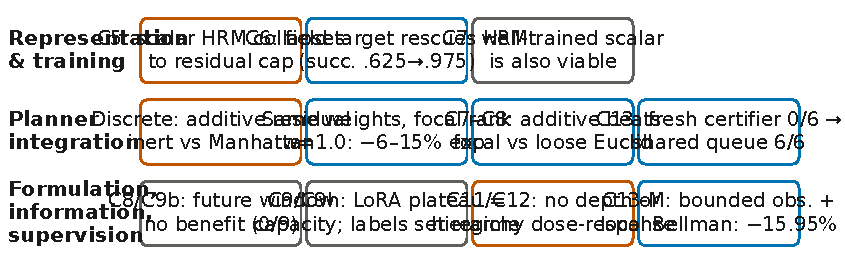
\includegraphics[width=0.98\textwidth]{figures/fig1_program_map.pdf}
\caption{The three harness layers, with the stages that intervened at each layer and their verdicts (orange: failure or negative; blue: positive under the corrected harness; gray: mechanism or null result). Reading down the columns: apparent architecture failures were repaired without changing the architecture (\stage{C6}, focal ranking, shared-queue certification), while apparent architecture advantages did not survive controls at the formulation layer (\stage{C11}, \stage{C12}). The constructive endpoint (\stage{C13-M}) changes only information access and integration.}
\label{fig:map}
\end{figure*}

\section{Benchmark Ladder and Methodology}

\textbf{Substrate.} A point robot plans through 2-D worlds via a PRM ($\sim$192 nodes, $k{=}7$) with A\textsuperscript{*} \citep{hart1968astar} under a per-suite \emph{binding budget} of expansions. Training labels are exact graph-Dijkstra costs (static), exact backward space--time Dijkstra values over $(\text{node},t)$ states (dynamic; cf.\ space--time search \citealp{silver2005cooperative,phillips2011sipp}), or---in the final stage---behavior-derived returns that never read shortest-path values. Learned providers include scalar regressors and goal-conditioned raster \emph{value fields} sampled at PRM nodes, over HRM, ON-LSTM \citep{shen2019onlstm}, LSTM \citep{hochreiter1997lstm}, U-Net \citep{ronneberger2015unet} with FiLM conditioning \citep{perez2018film}, graph networks, MLPs, and a faithfully ported HRM-v2 with adaptive computation \citep{graves2016act,banino2021pondernet}. A discrete-grid counterpart (20$\times$20 to 256$\times$256, Manhattan baseline) provides the cross-domain contrast.

\textbf{Metrics.} We separate \emph{success} at the binding budget (paired McNemar tests, Benjamini--Hochberg corrected) from \emph{matched-solved expansion ratios} (learned/baseline on worlds both solve; bootstrap CIs), and report path suboptimality separately, following the observation that aggregate point estimates without paired uncertainty mislead \citep{henderson2018matters,agarwal2021precipice}.

\textbf{Calibration and headroom gates.} Early stages saturated: at budget 100 the Euclidean baseline already solved 92.5--100\% of nine pilot suites, hiding all differences. Stage \stage{C5} therefore \emph{calibrated} map difficulty until the baseline fell into a discriminative band (0.25--0.62 success). Later stages generalize this into explicit authorization gates: \stage{C11} required an exact compositional oracle to clear a preregistered advantage gate over a leg-sum baseline (oracle/leg-sum expansion ratio $\leq$0.5--0.6) before any architecture arm was trained---observed ratios were 0.082--0.225; \stage{C12} required proof that hidden-regime histories are decision-relevant (71.3\% aliased decisions; a privileged-history diagnostic worth $+0.467$ completion) before testing learned memory; \stage{C13} established oracle integration ceilings before inserting any learned provider. A null under a passed headroom gate is informative; without one it is noise.

\textbf{Preregistration and integrity.} From \stage{C7} onward, designs, gates, budgets, and analysis grains were frozen before runs; artifacts are hash-bound; confirmation cohorts are generated only after model and integration are frozen; failed development gates block confirmation rather than triggering retuning \citep[cf.][]{pineau2021reproducibility}. Two validity catches justify the machinery (forensics in the technical appendix): a celebrated adaptive-computation accuracy metric that was exactly $100$ minus exact-match accuracy---a frozen, constant-false halt head---and a continuity check whose failure was diagnosed as a false premise rather than a measurement bug.

\section{Layer I: Representation and Training}

On calibrated hard maps (\stage{C5}), a pooled ON-LSTM scalar regressor was strong---hard-maze success 0.525$\to$1.000 over Euclid ($q{=}4.3{\times}10^{-11}$), dense maze 0.595$\to$0.962---while scalar HRM \emph{collapsed to a constant} at the residual cap and matched the baseline exactly; lower learning rates and a differentiable soft cap reproduced the collapse. Read naively, this is ``hierarchy fails where recurrence succeeds.''

\stage{C6} changed only the representation and objective: predict a goal-conditioned raster residual \emph{field}, sample it at PRM nodes. HRM's success rose 0.625$\to$0.975 ($q{=}3.4{\times}10^{-4}$; $-42.4$ mean expansions), alongside U-Net (0.950) and ON-LSTM (0.900). The failure was the harness, not the model. The converse over-read is also blocked: \stage{C7} later trained scalar models properly and found scalar-HRM ratios of 0.427--0.822, equal or better than fields in several suites---so ``value fields are necessary'' is false as well. What \stage{C5}/\stage{C6} establish is that representation and optimization can single-handedly manufacture an architecture verdict in either direction.

\section{Layer II: Planner Integration}

\begin{figure}[t]
\centering
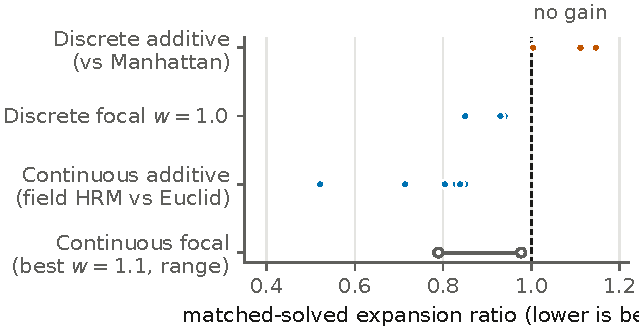
\includegraphics[width=0.98\columnwidth]{figures/fig2_integration.pdf}
\caption{The integration inversion. Against a \emph{tight} admissible baseline (discrete, Manhattan), additive learned magnitude is inert or harmful (ratios $\geq$1) while the same frozen weights win 6--15\% as a focal tie-breaker at $w{=}1.0$. Against a \emph{loose} baseline (continuous hard PRMs, Euclid), additive magnitude wins 15--48\% (field-HRM per-suite ratios shown) while the best post-hoc focal variant ($w{=}1.1$) recovers less (range bar).}
\label{fig:integration}
\end{figure}

\textbf{Continuous, loose baseline.} On \stage{C7}'s six hard static suites, additive learned heuristics dominate: field-HRM matched-solved ratios 0.521--0.850 (significant success gains in 4/6 suites after correction), scalar-HRM 0.427--0.822, at path suboptimality $\approx$1.02--1.14. Focal variants \citep{pearl1982semiadmissible}---which preserve a $w$-bound \citep{pohl1970}---recover far less (best post-hoc $w{=}1.1$ ratios 0.789--0.977). Under \stage{C8}'s deterministic moving obstacles with exact space--time labels, the pattern repeats at larger scale: selected learned arms cut matched expansions 62--95\% (ratios 0.046--0.380) with success gains of $+0.2$ to $+0.7$ (5/6 suites significant, corrected), and additive again beats focal.

\textbf{Discrete, tight baseline.} The discrete program inverts this. A pooled learned residual is a near-perfect \emph{ranker} (correlation with the true residual 0.987--0.994 across map sizes) whose \emph{magnitude} is scale-flat: predicted/true means fall from 0.73 at 64$\times$64 to 0.19 at 256$\times$256. Injected additively against Manhattan, it is inert or harmful (in a controlled 22-suite run, every learned arm $\leq$ baseline). Moved---frozen---into a focal band at $w{=}1.0$, the same weights cut expansions 6--15\% with no observed success regression. This vindicates ranking-based training arguments \citep{chrestien2023rank} from the integration side: the information was present all along; the planner was consuming the wrong aspect of it.

\textbf{The principle.} \emph{Diagnose the baseline before choosing the integration.} When the admissible baseline is loose, additive learned magnitude buys large reductions at bounded suboptimality cost; when it is tight, only within-band ranking is safe and useful (Figure~\ref{fig:integration}).

\textbf{A microcosm with an oracle.} \stage{C13} replays the principle with the true value function. A learned-incumbent search followed by a \emph{fresh} certifier search loses all six test worlds at $w{=}1.10$ \emph{even when the incumbent is the oracle} (total 141.2 vs.\ 129.7 expansions for matched focal): the certifier discards the incumbent's work. Sharing a single queue and $g$-state---changing nothing else---wins all six (122.8 vs.\ 129.7). An integration can erase an oracle; no architecture conclusion drawn upstream of such a repair is safe.

\section{Layer III: Information and Supervision}

\begin{figure}[t]
\centering
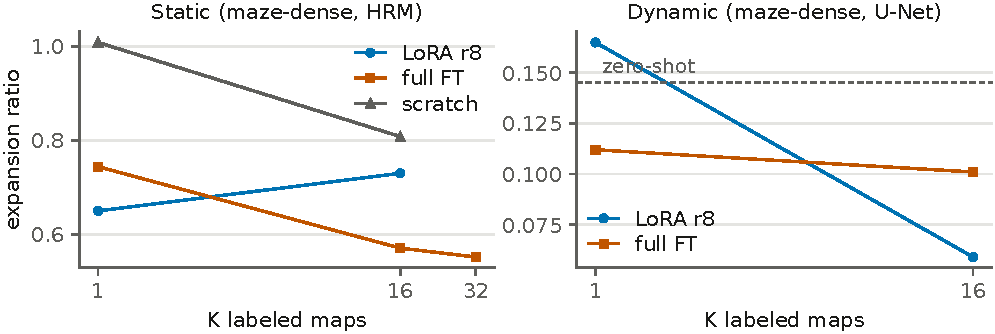
\includegraphics[width=0.98\columnwidth]{figures/fig3_transfer.pdf}
\caption{Supervision density sets the transfer regime (HRM/U-Net examples; matched-solved ratio vs.\ $K$ labeled target worlds, recorded points only). Left: with scarce static labels, rank-8 LoRA preserves the pooled base at $K{=}1$ while full fine-tuning is unstable early and wins by $K{=}16$--$32$. Right: one dynamic world already supplies $\sim$25k $(\text{node},t)$ labels, and the crossover disappears. Points are the canonical record-level curve medians; world-clustered CIs confirm both regimes (technical appendix).}
\label{fig:transfer}
\end{figure}

\textbf{Future information: a twin-control null.} \stage{C8} trains aware/blind twins differing only in an 8-step future obstacle window. Across 24 suite$\times$backbone cells, seven uncorrected significant cells favor \emph{blind}, one favors aware; direct heuristic accuracy splits 11/24 vs.\ 13/24. Adaptation does not unlock the window either: at full fine-tuning with $K{=}16$ in \stage{C9b}, no cell shows a significant aware advantage---world-clustered deltas span $-0.050$ to $+0.017$, eight of nine point deltas are zero or negative, and all nine CIs cross zero. We claim no systematic benefit---not harm, and not equivalence.

\textbf{Adaptation: capacity, not clamps.} Few-shot transfer of pooled bases to held-out families (\stage{C9}) shows rank-8 LoRA \citep{hu2021lora} preserving a strong base at $K{=}1$ (e.g., maze-dense ratio 0.650 at success 1.00) while full fine-tuning is high-variance early and reaches lower ratios given labels ($0.571$ at $K{=}16$; rooms-large $0.500$ at $K{=}8$); training from scratch is far behind at low $K$. These orderings are world-clustered-significant: at the corrected grain, full fine-tuning at $K{=}16$ (ratio $0.610$ $[0.549,0.670]$) beats LoRA ($0.786$ $[0.694,0.891]$) with disjoint CIs, the rooms-large $K{=}1$ catastrophe sits entirely above parity ($1.293$ $[1.170,1.503]$), and LoRA's bugtrap degradation at $K{=}32$ is significant (appendix). A matched-compute dissection (\stage{C9h}) attributes the LoRA plateau: bounded and unbounded rank-8 adapters differ by a median ratio delta of $0.000\pm0.008$ across 27 cells---the plateau is \emph{low-rank capacity}, not the output bound. The strongest single cell is architecture-agnostic in the telling direction: a field U-Net moves from 0.982 zero-shot to 0.404 under full fine-tuning while its conv-LoRA stays at $\approx$0.99.

\textbf{Labels, not worlds, define the regime.} Under dynamics (\stage{C9b}), one world supplies $\sim$25{,}000 supervised $(\text{node},t)$ states; full fine-tuning is no longer catastrophic at $K{=}1$ and the static crossover disappears (Figure~\ref{fig:transfer}). Transfer still dominates scratch. The regime variable is supervision density---a caution for ``few-shot'' claims indexed by task count.

\textbf{Composition: a null with working machinery.} Zero-label interpolation of 16 family experts by task-descriptor RBF weights (\stage{C10}) routes almost perfectly (own-axis mass 0.986--0.998) yet never significantly beats the pooled zero-shot base and is significantly \emph{worse} in two of six cells under world-paired reanalysis (published deltas $-0.024$ to $+0.116$; worst clustered delta $+0.098$ $[+0.076,+0.123]$; uniform mixing often matches RBF)---separating ``routing works'' from ``composition pays,'' and consistent with weight-space merging accounts \citep{wortsman2022soups,ilharco2022task}.

\section{The Hierarchy Audit}

\begin{figure}[t]
\centering
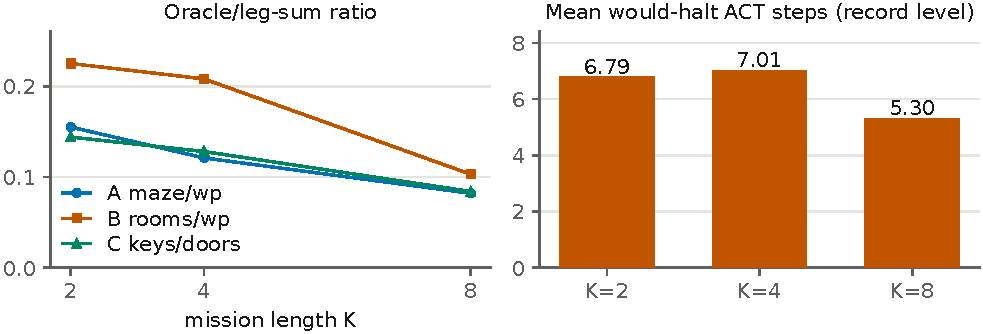
\includegraphics[width=0.98\columnwidth]{figures/fig4_c11.pdf}
\caption{\stage{C11}. Left: the exact compositional oracle's expansion ratio over a leg-sum baseline \emph{falls} with mission length $K$---headroom for depth-exploiting guidance grows. Right: HRM-v2's learned halting spends \emph{fewer} adaptive-computation steps on deeper missions ($\rho{=}-0.407$, permutation $p{\approx}5{\times}10^{-4}$, $n{=}675$)---the opposite of the depth-of-compute hypothesis.}
\label{fig:c11}
\end{figure}

\stage{C11} was designed \emph{for} hierarchy to win: compositional missions (multi-waypoint and key/door tasks, length $K\in\{2,4,8\}$) whose exact oracle enjoys 4--12$\times$ headroom over a sum-of-independent-legs baseline, global map/graph inputs for every arm, six matched architectures (MLP, FiLM U-Net, product-graph GNN, HRM trace, ON-LSTM trace, HRM-v2 with adaptive computation), three seeds, 198 checkpoints, 54{,}450 evaluation rows. The preregistered outcomes were negative on every hierarchy-specific gate. No structured arm beats the MLP at two mission depths with a non-decreasing gap (G1). Forcing HRM-v2 to spend $k{=}1/2/4/8$ recurrent segments leaves expansion and error curves flat (G2a). Learned halting \emph{inverts}: mean would-halt steps are 6.79/7.01/5.30 at $K{=}2/4/8$, and the anti-correlation \emph{strengthens} at the world-clustered grain ($\rho{=}-0.58$, stratified permutation $p{=}5{\times}10^{-5}$, $n{=}225$; Figure~\ref{fig:c11}). What \emph{did} appear is an information-structure effect: the global-input U-Net and GNN beat the MLP at shallow $K$ (versus-MLP ratios $\approx$0.67--0.87; state-value MAE 0.151/0.171 vs.\ 0.251 at config A, $K{=}0$; world-clustered CIs exclude parity at $K\in\{0,2\}$ in two of three configs)---an advantage that dissolves by $K\in\{4,8\}$, where every cell's CI includes parity. Five of 33 recurrent cells exhibit constant-prediction collapse (a reproducible loss signature; removing padding \emph{worsens} recurrent predictions, showing models were exploiting pad steps as extra compute), so the worst recurrent cells are optimization pathology, not capacity estimates. A 12-run scaled addendum preserves the ordering (U-Net completion 0.804 vs.\ HRM 0.736 at $K{=}2$; 0.413 vs.\ 0.307 at $K{=}8$, where HRM exactly matches the leg-sum baseline---persistent collapse).

\stage{C12} tested two rescue hypotheses. (i) \emph{Persistent memory}: with proven headroom (see Methodology), a matched temporal-hierarchy pilot still fails forecast, planning, and state-carry gates---\emph{strong negative}. (ii) \emph{Iterative depth}: a tied product-graph refiner improves bounded-search burden monotonically with cycles in \emph{every} cell (e.g., C/$K{=}8$: 0.576$\to$0.517 normalized burden, cycle 1$\to$8)---recurrent compute genuinely helps---but the gain is no larger at $K{=}8$ than $K{=}2$ (the preregistered dose--response fails; $K8{-}K2$ deltas $+0.004$ and $-0.031$, CIs crossing zero), and weight tying wins only one configuration ($q{=}6.7{\times}10^{-5}$) while losing the other. Value diagnostics sharpen the reading: Bellman residuals \emph{worsen} over cycles while search burden improves---the refiner is learning search efficiency, not value iteration \citep[cf.][]{tamar2016vin,lee2018gppn}.

\stage{C13-N/O} close the loop under a \emph{working} method (next section): substituting a trimmed HRM for the successful MLP retains useful pooled signal ($-8.6$ expansions vs.\ the field baseline, CI $[-16.7,-1.2]$) but fails suite-robustness and path-quality gates; moving the summary token to the final readout position helps transiently at one checkpoint and fails at the endpoint. Where forecasting-style tasks \emph{did} separate architectures (discrete dynamic-obstacle prediction), the sign was task-dependent---HRM 71/100 vs.\ LSTM 68--69/100 on one protocol; ON-LSTM 0.388 vs.\ HRM 0.265 mean success on a harder structured protocol---and never uncertainty-quantified hierarchy evidence. Our conclusion is deliberately bounded: \emph{no tested formulation converts nominal hierarchy or added depth-of-compute into a growing advantage on deeper or more compositional planning problems}; where architecture matters, information structure (global views, gated recurrence on genuinely temporal signals) is the operative ingredient.

\section{A Constructive Inversion: Less Information, Better Integration}

\begin{figure*}[t]
\centering
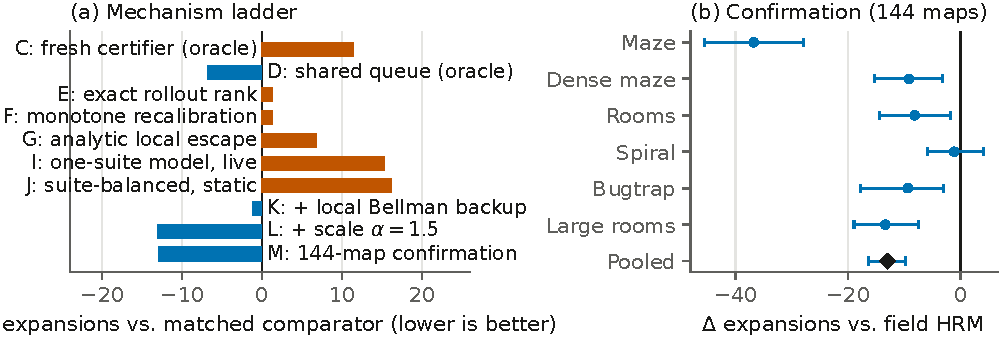
\includegraphics[width=0.98\textwidth]{figures/fig5_c13.pdf}
\caption{\stage{C13}. (a) The mechanism ladder: each rung changes one factor; bars are paired expansion deltas versus the matched comparator (rungs C--G versus matched focal search at $w{=}1.10$, including \emph{oracle} providers; rungs I--M versus the preregistered complete-map comparator, field HRM, live on all six suites). Target repairs and distribution repairs fail; one radius-bounded inference-time Bellman backup (K) plus scale calibration (L) flip the sign. (b) Preregistered confirmation on 144 untouched worlds: pooled delta $-12.96$ expansions (95\% CI $[-16.30,-9.74]$; 109 wins/3 ties/32 losses), every suite mean negative, at matched empirical path quality.}
\label{fig:ladder}
\end{figure*}

The program's endpoint inverts a constraint into a result. Motivated by real-time search's state-local tradition \citep{korf1990rta,koenig2006rtaa}, the final stage restricts the heuristic for state $s$ to \emph{bounded local observations} around $s$ on a known PRM---no complete-map raster, no shortest-path supervision, labels derived from fresh-start local-policy rollouts. The preregistered primary comparator is \stage{C7}'s headline provider, the complete-map field HRM; every other \stage{C7} learned provider is also recomputed live.

The ladder (Figure~\ref{fig:ladder}a) isolates the mechanism one variable at a time. The exact behavior-return statistic, replayed with no model error, is $+1.3$ expansions worse than matched focal search---and monotone recalibration does not fix it: the \emph{target}, not model capacity, is the first blocker. Analytic radius-bounded escape constructions are valid but too weak ($+6.8$). A model trained on one suite fails across the distribution ($+15.4$, CI $[+12.0,+18.6]$); suite-balanced retraining \emph{still} fails when inserted statically ($+16.2$): distribution repair alone is insufficient. The decisive change is a single radius-bounded Bellman backup at inference, using learned predictions only as local exit values---the same checkpoint moves from $+16.2$ to $-1.2$, and scale calibration ($\alpha{=}1.5$ on 48 fresh worlds) reaches $-13.0$ (CI $[-18.7,-7.6]$) with all six suite means negative.

Everything was then frozen---model, radius 0.20, $\alpha{=}1.5$, integration, gates---before generating 144 zero-overlap confirmation worlds (24 per suite). The bounded-observation arm expands 68.31 nodes on average versus 81.26 for field HRM: paired delta $-12.96$, bootstrap 95\% CI $[-16.30, -9.74]$, 109/3/32 win/tie/loss, all six suite means negative (Figure~\ref{fig:ladder}b; Table~\ref{tab:c13m}), with \emph{better} empirical path-cost ratios (mean/max 1.024/1.162 vs.\ 1.031/1.335). The confirmed arm also beats \emph{every} fixed \stage{C7} learned provider in pooled expansions on this cohort. A separate $w{=}1.10$ reopening-focal operating point returns 144/144 valid paths with zero bound or certificate violations, cleanly separating the matched-quality direct arm from the formally bounded control.

Three caveats travel with the number. The direct arm carries no formal suboptimality bound (the bounded control does). The unoptimized Python feature builder averages 5.14\,s/world versus 0.37\,s for field-HRM inference---this is a search-expansion and path-quality result, not a wall-clock one (model inference itself is 0.8\,ms). And it is one model seed and one confirmation cohort. Under those caveats the lesson stands: a model that \emph{sees less} but is integrated so that inference performs the right local computation---one Bellman backup, kin to a single VIN iteration \citep{tamar2016vin} applied at the planner interface---beats models that see everything. Architecture substitutions under this same working method (\stage{C13-N/O}, above) do not preserve the gain, underlining that the mechanism is the harness, not the backbone. A follow-up testing genuinely persistent planning-time state (carry across a query's expansion sequence, against a same-checkpoint reset twin) is preregistered with a verified harness and executing at the time of writing; its integrity gates have not yet passed, and it contributes no outcome evidence here.

\begin{table}[t]
\centering
\small
\begin{tabular}{lcc}
\toprule
 & Bounded-obs.\ (ours) & Field HRM \\
\midrule
Mean expansions $\downarrow$ & \textbf{68.31} & 81.26 \\
Paired $\Delta$ [95\% CI] & \multicolumn{2}{c}{$-12.96$ $[-16.30,\,-9.74]$} \\
Win / tie / loss & \multicolumn{2}{c}{109 / 3 / 32} \\
Suite means negative & \multicolumn{2}{c}{6 / 6} \\
Mean cost ratio $\downarrow$ & \textbf{1.0235} & 1.0311 \\
Max cost ratio $\downarrow$ & \textbf{1.1624} & 1.3346 \\
Valid paths & 144 / 144 & 144 / 144 \\
Feature build (s/world) $\downarrow$ & 5.138 & \textbf{0.371} \\
\bottomrule
\end{tabular}
\caption{\stage{C13-M} preregistered confirmation on 144 untouched worlds (24 per suite; one model seed). Cost ratios are relative to graph-optimal cost. A separate $w{=}1.10$ reopening-focal control passes all 144 safety certificates. Bold marks the better value.}
\label{tab:c13m}
\end{table}

\begin{table*}[t]
\centering
\footnotesize
\begin{tabular}{@{}p{1.5cm}p{3.3cm}p{3.6cm}p{8.0cm}@{}}
\toprule
Stage & Protocol & Question & Verdict (headline evidence) \\
\midrule
\stage{C1--C4} & easy PRM pilots & do learned bases/experts help? & saturated; Euclid 0.925--1.00 success; specialists $\leq$3\% \\
\stage{C5} & calibrated hard maps, scalar & learned scalar guidance? & ON-LSTM $+0.48$ succ.\ ($q{=}4{\times}10^{-11}$); HRM collapses to cap \\
\stage{C6} & value-field target & does representation rescue HRM? & yes: 0.625$\to$0.975 succ.\ ($q{=}3.4{\times}10^{-4}$) \\
\stage{C7} & static integration matrix & additive vs.\ focal vs.\ scalar/field & additive wins vs.\ loose Euclid; ratios 0.43--0.85; subopt.\ 1.02--1.14 \\
\stage{C8} & space--time dynamics, twins & dynamic gains? future window? & ratios 0.046--0.380; no systematic aware benefit (7 blind vs.\ 1 aware) \\
\stage{Discrete} & grids, Manhattan baseline & additive vs.\ focal ranking & additive inert/harmful; same weights focal $w{=}1.0$: $-$6--15\% \\
\stage{C9/C9h} & few-shot static transfer & LoRA vs.\ full FT vs.\ scratch & LoRA preserves at $K{=}1$, plateaus by \emph{capacity} (bound $\Delta{=}0.000{\pm}.008$) \\
\stage{C9b} & transfer under dynamics & does the crossover persist? & no: $\sim$25k labels/world; 0/9 aware wins; transfer $\gg$ scratch \\
\stage{C10} & zero-label expert interpolation & does composition beat zero-shot? & null (deltas $-0.02$ to $+0.12$) despite 0.99 routing selectivity \\
\stage{C11} & compositional missions & hierarchy/depth dose--response? & hierarchy gates all negative; halting inverts ($\rho{=}-0.407$); shallow global-input wins \\
\stage{C12} & hidden regimes; tied refiner & memory? iterative depth? & pilot strong-negative; cycles help monotonically but no $K$ dose--response \\
\stage{C13-A--L} & bounded observation ladder & what blocks a local heuristic? & target, then distribution, then \emph{integration}; local backup flips $+16.2\to-1.2$ \\
\stage{C13-M} & frozen 144-world confirmation & does it beat complete-map field HRM? & yes: $-12.96$ exp.\ (CI $[-16.3,-9.7]$), matched path quality \\
\stage{C13-N/O} & architecture substitution & does HRM preserve the gain? & no: suite-robustness and path-quality gates fail; readout fix transient \\
\bottomrule
\end{tabular}
\caption{The program at a glance. Every verdict is stated at the strength its evidence supports (local single-GPU validations; see Limitations). Full per-suite tables, protocols, and statistics appear in the technical appendix.}
\label{tab:matrix}
\end{table*}

\section{Related Work}

\textbf{Learned heuristics and guidance.} Bootstrapped heuristic learning \citep{arfaee2011bootstrap}, imitation of clairvoyant oracles \citep{bhardwaj2017sail}, differentiable search \citep{yonetani2021neuralastar}, transformer heuristics for grids \citep{kirilenko2023transpath}, and supervised heuristics for classical planning \citep{ferber2020neural} all report guidance gains; our contribution is orthogonal---controlling the harness those gains ride on. Our focal result gives integration-side support to the argument that heuristics should be optimized (or here, consumed) as \emph{rankings} rather than cost estimates \citep{chrestien2023rank}. Bounded-suboptimal search supplies the integration vocabulary \citep{pohl1970,pearl1982semiadmissible}, and multi-heuristic scheduling \citep{aine2016mha} is the natural home for unreliable learned signals we did not explore. The final stage's state-local restriction descends from real-time heuristic search \citep{korf1990rta,koenig2006rtaa}; its one-backup integration is kin to value-iteration modules \citep{tamar2016vin,lee2018gppn} and, more broadly, to executing the right algorithmic step inside a learned system \citep{velickovic2021nar}.

\textbf{Hierarchical and recurrent reasoning models.} HRM \citep{wang2025hrm} motivates our central question; recursive tiny networks \citep{jolicoeur2025trm} independently found that much of HRM's benchmark performance survives drastic architectural simplification. We add controlled planning-side evidence: favorable-condition headroom, forced-compute and halting gates, collapse forensics, and substitution tests under a working method. Learned subgoal hierarchies \citep{czechowski2021subgoal} remain a distinct, planner-side route to hierarchy that our formulation-level negative does not address.

\textbf{Motion planning and learning.} PRMs \citep{kavraki1996prm} and learned samplers/planners \citep{ichter2018sampling,qureshi2019mpnet} define the continuous substrate tradition; space--time search under moving obstacles follows \citet{silver2005cooperative} and \citet{phillips2011sipp}.

\textbf{Adaptation and evaluation practice.} LoRA \citep{hu2021lora} and weight-space composition \citep{wortsman2022soups,ilharco2022task} frame our transfer and interpolation results. Our statistics and preregistration discipline follow the reproducibility literature \citep{henderson2018matters,agarwal2021precipice,pineau2021reproducibility}.

\section{Limitations}

Headline continuous results are local, single-GPU validations with one primary training seed each; stages share trained bases and evaluation worlds and are not independent replications. Several stages (\stage{C9}--\stage{C11}) originally pooled repeated evaluations of the same test worlds across adaptation/model seeds; a world-clustered reanalysis of every quantity this paper quotes from those stages (technical appendix) flips no verdict---it strengthens the halting inversion and the composition negative, adds CIs to the transfer orderings, and softens one phrasing (\stage{C9b})---but the full-grid refresh of all published tables remains for the camera-ready. \stage{C13-M} is one model seed and one confirmation cohort; its direct arm carries no formal bound (the separate focal control does), its feature construction is currently slower than field-HRM inference in wall time, and its observation model assumes a known PRM rather than map-free sensing. All negatives are failures to observe an effect under specified conditions---not equivalence claims, and not claims that hierarchy can never help planning; the persistent-state follow-up is preregistered and still inside its integrity gates, contributing no evidence. Benchmarks are 2-D single-agent point-robot worlds; external validity beyond this substrate is untested.

\section{Conclusion}

Across thirteen preregistered stages and two substrates, the payoff of learned search guidance was governed---start to finish---by the harness: what the model is asked to predict, where its output enters the planner, what information it may see, and how much supervision defines its regime. Architectural hierarchy, tested under conditions engineered in its favor, never converted depth into advantage; restructuring the harness converted a constraint into the program's strongest result. For practitioners we distill a checklist: calibrate the benchmark until the baseline can lose; prove headroom with an oracle before comparing architectures; diagnose baseline tightness before choosing additive or ranking integration; match supervision density before naming a transfer winner; and treat every training collapse as a validity bug until proven otherwise. For the architecture debate we offer a falsifiable standard: a hierarchy claim on planning should survive exactly the gates that dissolved ours.

\bibliography{references}

\end{document}
